\documentclass{sig-alternate-05-2015}
\usepackage{cite}
\usepackage{amsmath}
\usepackage{tcolorbox}
\usepackage{pdfpages}
\usepackage{hyperref}

\newcounter{qcounter}


\begin{document}

% Copyright
\setcopyright{acmcopyright}

% DOI
\doi{10.475/123_4}

% ISBN
\isbn{123-4567-24-567/08/06}

%Conference
\conferenceinfo{EMSE '16}{March 28--June 10, 2016, Corvallis, OR, USA}

\acmPrice{\$15.00}

\title{(Merge) Conflicts of Interest: Resolution Patterns in Practice}
\subtitle{Midterm Report for Empiricial Methods of Software Engineering (EMSE), Spring 2016}

\numberofauthors{2}

\author{
\alignauthor
	Shane McKee\\
       	\affaddr{Oregon State University}\\
       	\affaddr{2500 NW Monroe Avenue}\\
       	\affaddr{Corvallis, Oregon}\\
       	\email{mckeesh@oregonstate.edu}
\and
\alignauthor
Nicholas Nelson\\
       \affaddr{Oregon State University}\\
       \affaddr{2500 NW Monroe Avenue}\\
       \affaddr{Corvallis, Oregon}\\
       \email{nelsonni@oregonstate.edu}
}


\maketitle
\section{Introduction}\label{Introduction}
Collaboration between software developers working on the same project also carries the risk of merge conflicts. With 28.4\% of all projects on Github being non-personal repositories (as of Jan. 2014), the prevalence of merge conflicts is significant \cite{kalliamvakou14}. Since merge conflicts carry a cost to any software project, developers and researchers have pursued ways of mitigating them \cite{niu2012}. But mitigation strategies must be based upon a foundation of understanding both the problem space --- conflicting versions of code --- and the factoring that contribute to their occurrence.

Popular version control systems (git, svn, etc.) have features that allow for the detection of merge conflicts, and can automatically resolve the conflict when it adheres to certain basic patterns of textual conflicts. But when more complex conflicts occur, either in the form of syntactic or semantic conflicts, these version control systems require developer intervention to resolve the conflict. Although several papers have examined how and why merge conflicts occur \cite{brun10}\cite{Sarma08}\cite{Guimaraes12}, little attention has been paid to understanding how developers resolve merge conflicts in practice.

By mining software repositories on Github for instances of merge conflicts, we hope to characterize the patterns that developers take to resolve merge conflicts. When examined across the backdrop of tools in use for managing code, our data will show whether the features of these tools are adequately addressing the needs of software developers collaborating within open-source communities.

\begin{table*}
\centering
\caption{Executive Summary}
\begin{tabular}{| l | p{10cm} | } \hline
Goal & To understand merge conflict resolution patterns in Git repositories. \\ \hline
Research Questions  & \textbf{RQ1:} What merge conflict resolution patterns exist in Git?\\
& \textbf{RQ2:} What is the frequency distribution of merge conflict resolution patterns by programming language?\\
& \textbf{RQ3:} Is there a relationship between the size of the conflict and its conflict resolution pattern?\\ \hline
Empirical Method & This project will use data mining. Data mining is best for RQ1 because it will give us the least biased view of what developers do to resolve conflicts in practice. It is best for RQ2 because It will allow us to get a sample across a wide variety of languages while testing for certain resolution patterns. It is best for RQ3 because it is easy to extract the size of a conflicted area and compare it to the type of merge conflict resolution that was used.\\ \hline
Data Collected & Number of merges, number of merge conflicts, size of each conflict, pattern used in each resolution, primary programming language of each project, author of each original commit, parent commit, and merged commit\\
\hline\end{tabular}
\label{table:t1}
\end{table*}

\section{Background}\label{Background}

The underlying structure of version control systems affects the ways in which people interact with them. In this project, we focus on one aspect of the interactions with version control systems, but we provide a brief introduction to the structure as a background to our work.

Modern version control systems base their representations of code, and the underlying changes upon it, on graph theory. These models provide an entire family of models and methods for evaluating and attempting to resolve merge conflicts, but are limited either by the bounds of a particular model or the accuracy of its heuristics \cite{ehrig15} \cite{mens99}. We base our assumption that certain merge conflicts cannot be resolved by version control systems, and thus require human intervention, on these fundamental limitations in graph modeling.

Merge algorithms are an area of active research, and consequently there are many different approaches to automatic merging, with subtle differences. The more notable merge algorithms include three-way merge \cite{livshits07}, recursive three-way merge, fuzzy patch application \cite{brunet06}, weave merge \cite{nguyen07}, and patch commutation. These concepts form both a model of understanding and a lens for us to examine the differences between the theoretical models and real-world application.

Our research is guided by prior work into conflict detection and automated conflict resolution. Brun, et al. \cite{brun11}, ML Guim\~{a}raes, et al. \cite{Guimaraes12}, C Schneider, et al. \cite{schneider04}, and Dewan et al. \cite{dewan07} have all attempted to locate current and upcoming merge conflicts as early as possible in order to prevent them from occurring. We take the approach that some conflicts cannot be detected either by collaborator awareness or by proactively engaging automated merging tools, and that understanding how developers currently adapt to such situations is fundamental to developing tools that support such situations.\\

\section{Study Design}\label{design}
\subsection{Aspects of software development considered} 
\subsubsection{Motivations}
Merge conflicts have become a popular area of study, perhaps due to the importance of version control in the developer workflow or developers' dislike for resolving messy merge conflicts. Resolving a merge conflict can require extra time to understand how the two sets of new code should be integrated together.
\subsection{Dataset}
Our data was selected from open-source projects on GitHub. This publicly accessible data is convenient, but it does run the risk of results not being sufficiently generalizable to private code repositories. The following data was gathered:
\begin{enumerate}
\item \textbf{Number of merges}\\
	This is the total number of merges, both automatically and manually merged. The intent is to identify what percentage the merges in our corpus must be manually merged.
\item \textbf{Number of merge conflicts}\\
	This is the number of merge conflicts that can be found using Git and GitPython. This will limit us to textual merge conflicits.
\item \textbf{Size of each conflict}\\
	We will determine the size of a conflict between commit A and commit B by the following equation:\\ 
	$$\text{SLOC}(\text{git diff}(Original, A))$$
	$$+$$
	$$\text{SLOC}(\text{git diff}(Original, B))$$
\item \textbf{Pattern used to resolve each conflict}\\
	Each merge conflict resolution was classified as one of the following patterns:
	\begin{enumerate}
	\item\textit{Take One:} Changes from one parent commit are taken while changes from the other parent commit are discarded.
	\item\textit{Interweaving:} Changes are taken from both commits and interweaving the conflicting code.
	\item\textit{Decline:} No changes are taken from either parent commit, and no lines are added while resolving the merge conflict.
	\item\textit{Overwrite:} No changes are taken from either parent commit, and code is added while resolving the merge conflict.
	\item\textit{Other:} The pattern found did not fall into any of the four defined patterns. 
	\end{enumerate}
\item \textbf{Primary programming language of each project}\\
Primary language is determined based on GitHub's internal analysis, which is determined by the prevalence of the language in the project.
\item \textbf{Author of each original commit, conflicting commits, and merged commit}\\
We use Git's metadata for each commit to determine the author.
\end{enumerate}

\subsection{Data Gathering and Analysis}
Our dataset is comprised of project metadata and commits particular to instances of merge conflicts. This dataset was gathered from Github using the GitPython tool in the following steps:\\

\begin{enumerate}
\item Collect all of the merges in a repository
\item Locate merge conflicts by merging two commits
\item Get the conflicting parts (\textbf{Part A} and \textbf{Part B}) from each commit by parsing out unmerged sections
\item Find the resulting merge conflict resolution (\textbf{M}) by branching from one parent, merging the other into the branch, committing the resulting merge conflict, then taking the diff between the commit and the merge conflict resolution.
\item Classify Part A, Part B, and M for each merge conflict resolution and its parents.
\end{enumerate}

\begin{figure*}[t]
\caption{Miner Architecture}
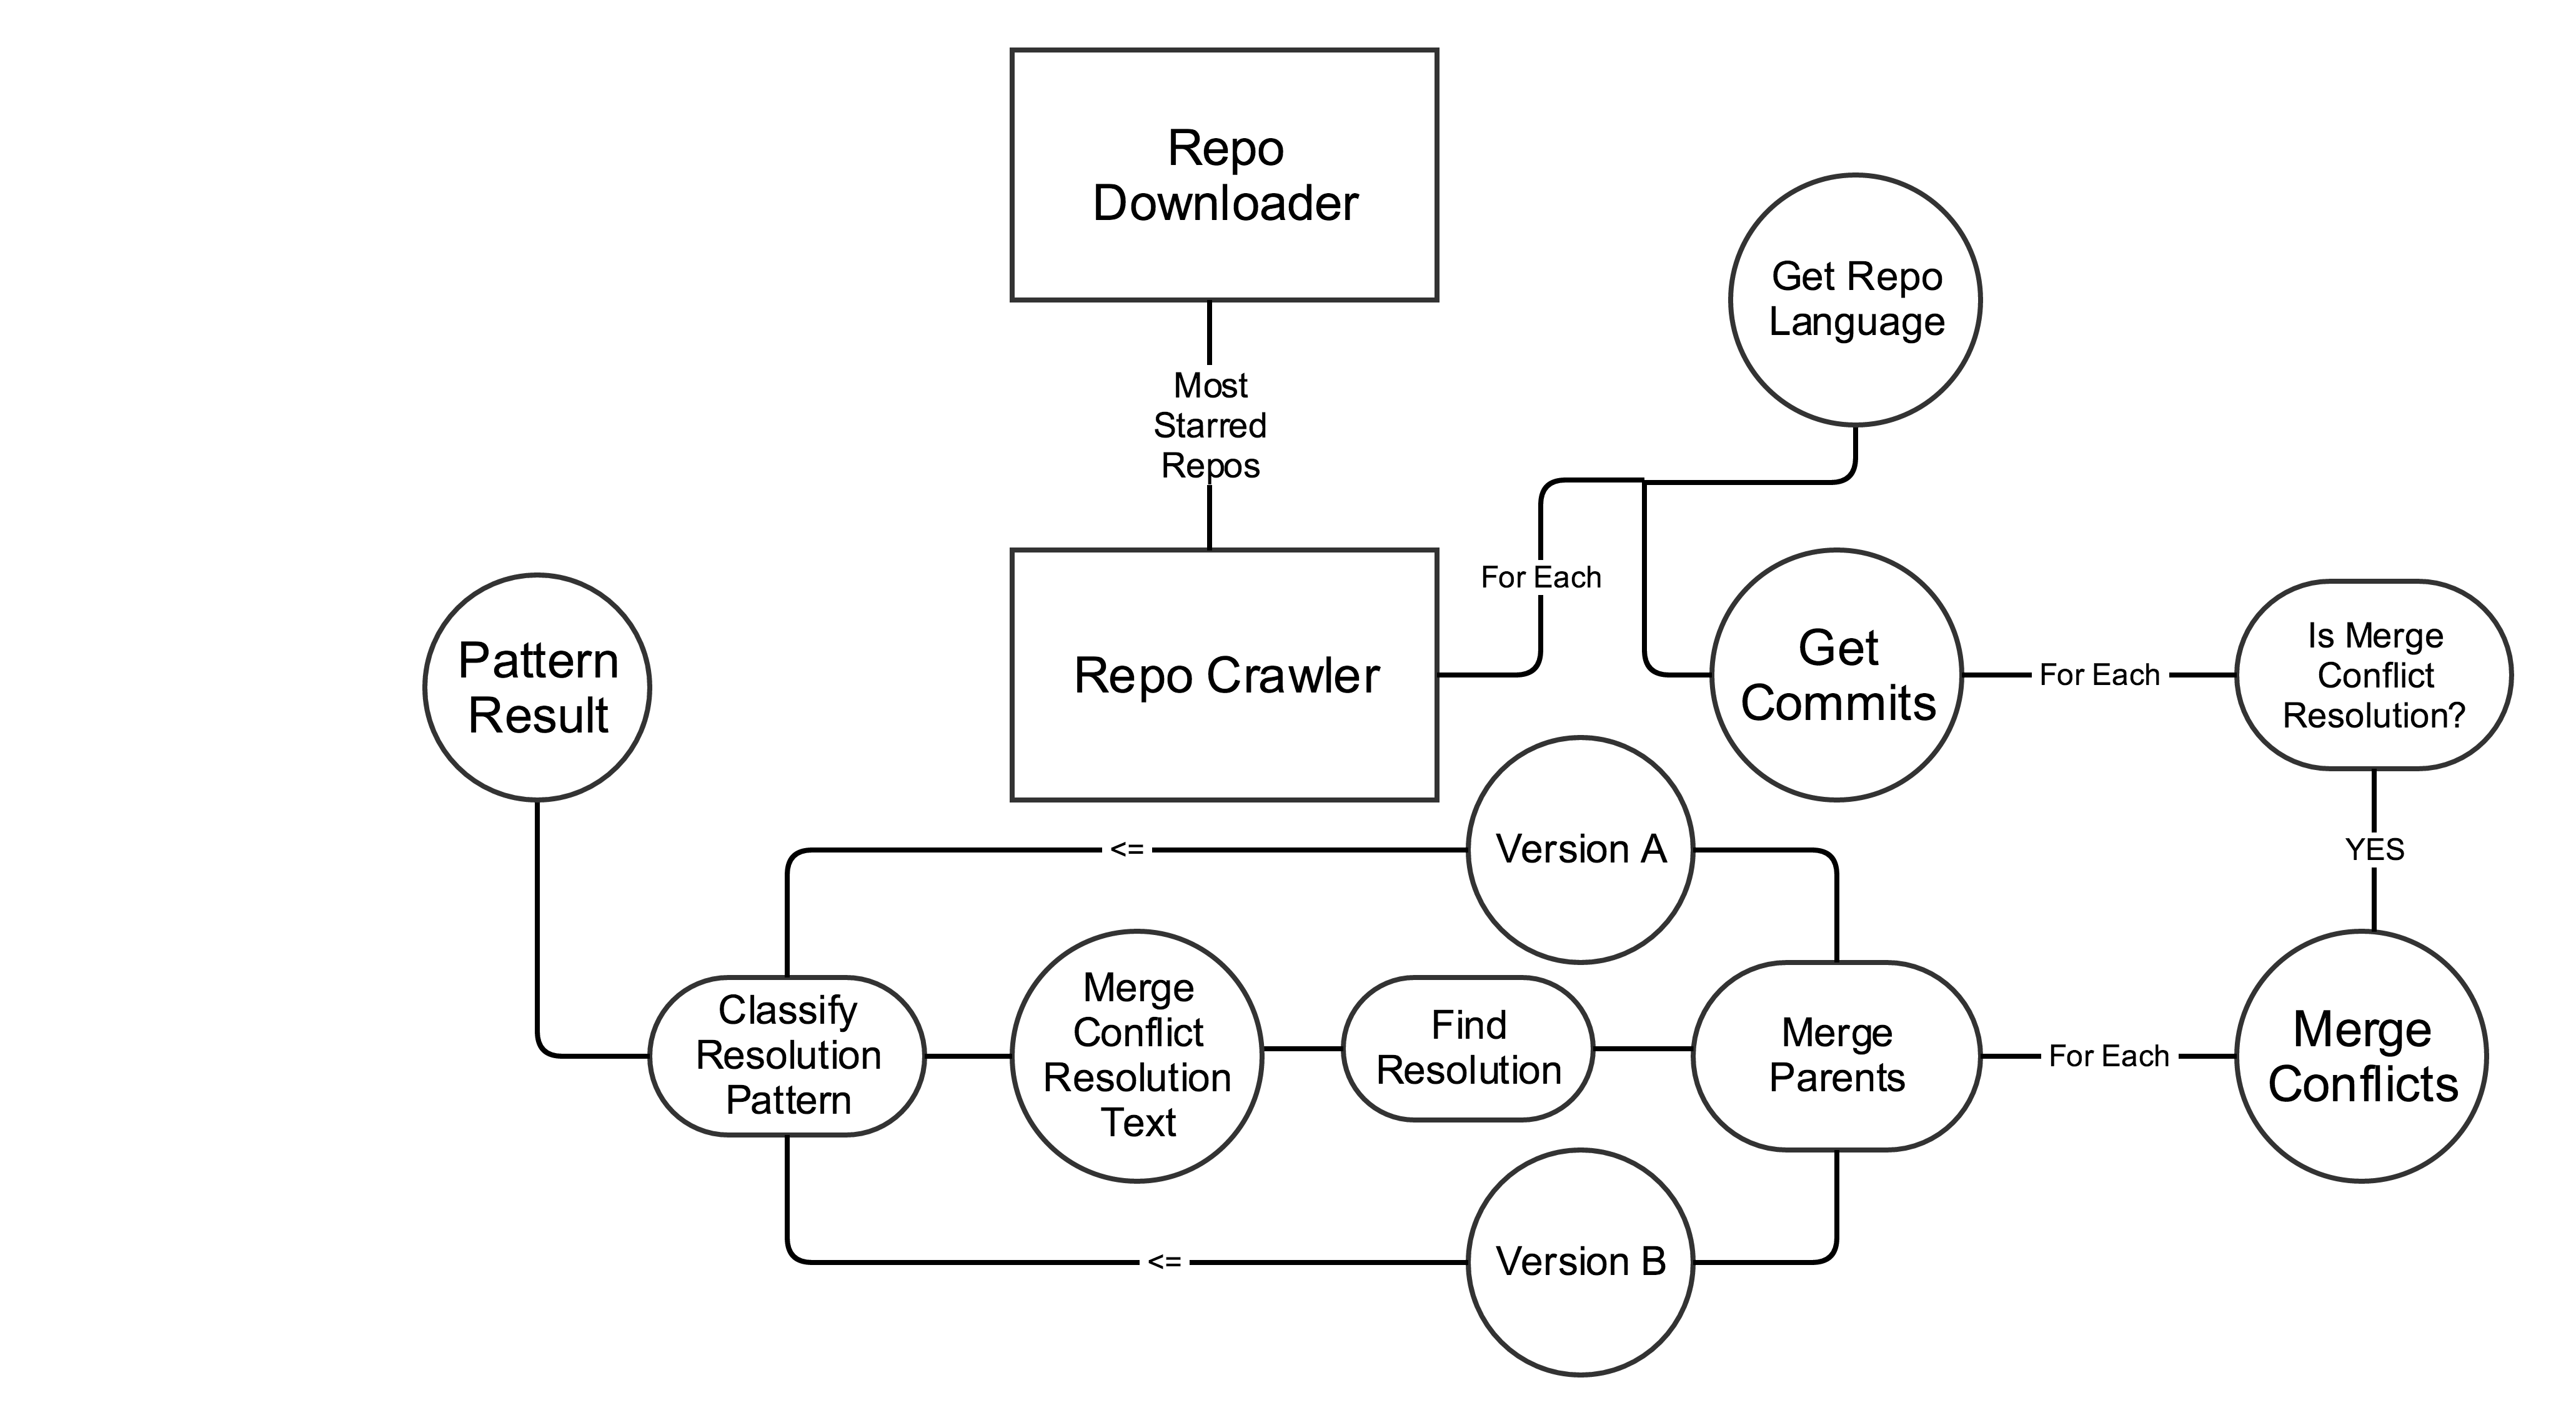
\includegraphics[width=\textwidth]{miningarchitecture}
\centering
\label{figure:f1}
\end{figure*}

The resulting dataset required manual pruning to remove some repositories. For instance, we found that many of the most starred repositories are tutorials, code camps, or just are not projects for software development.

Our study will be limited by both space and time. Since we must store the project metadata and each target commit while mining a Github repository, and retain any set of commits that are determined to be merges, we will be bound by the storage capacity of the system we use. The constraints of the term also introduces a time limitation to our project, but we should be able to mine a large enough dataset for determining initial results.

\section{Formative Results}\label{Results}
Though we have not yet collected any mining data, we do have an understanding of what characteristics we should expect to see. Outside of this project, one researcher has interviewed 9 software engineers about the types of merge conflicts that they encounter and how they resolve them. This has provided a better understanding about the type of data that we are looking for during the repository mining.

\section{Threats to Validity}
\textbf{Generalizability}
The project was run on a small set of projects, which may not be representative of all projects on GitHub.


\bibliography{references}{}
\bibliographystyle{plain}

\end{document}
